\chapter{Softwaretest}\label{sec:Softwaretest}
Der Softwaretest umfasst eine Nachweisstrategie und die Vorgaben der Entwicklung, um eine hochwertige Anwendung zu erstellen.

Die Nachweisstrategie beschreibt die Anwendung von Unit-Test auf das Gesamtsystem, insbesondere die Festlegung des Einsatzes und das Code Coverage.

Vorgaben für die Entwicklungsumgebung umfasst die Konfiguration der Unit-Tests/ Code Coverage Tools und die Verwendung der Testergebnisse.

\section{Konzept zum Softwaretest}
Das Konzept umfasst das Testverfahren während der Entwicklung mit abschließender Testdokumentation.

Folgende Anforderungen stellt das Konzept an das Testverfahren
\begin{itemize}
\item	Jede Methode wird mit Unit-Tests getestet. 
\item	Die Unit-Tests werden begleitend zur Entwicklungsphase geschrieben und erweitert
\item	Abschließend decken die Unit-Tests mindestens 85\% der implementierten Methoden ab, Frameworks ausgenommen
\item 	Regelmäßiges Prüfen der Code Coverage
\end{itemize}

Während des Entwicklungsprozesses wurden die Unit-Test kontinuierlich vervollständigt und mittels Code Coverage geprüft, ob die Testabdeckung ausreichend ist.

Die Unit-Tests wurden mit Hilfe von Jasmine erstellt.  Mittels zwei HTML-Dateien  \textit{``UnitTestModel.html''} und \textit{``UnitTestControllerView.html''} werden die Tests integriert. Darin erhält \textit{``UnitTestModel.html''} die Tests für das Model. Und \textit{``UnitTestControllerView.html''} enthält die Tests für den Controller und die View sowie einer Kopie der \textit{indexTableau.html} Dateien um die Manipulation des DOM-Tree zu testen. In der Datei \textit{``UnitTestModel.html''} wird das Test-Framework Jasmine im head-Tag eingebunden (Listing \ref{lis:EinbildungModel}). Dagegen wird Jasmine in der Datei \textit{``UnitTestControllerView.html''} am Ende der Seite im  body-Tag eingebunden, da es notwendig ist, dass das Markup vollständig geladen ist, bevor mit den Test begonnen werden kann (Listing \ref{lis:EinbildungControllerView}).
\begin{lstlisting}[language=HTML, caption= Einbildung Jasmine und Test-Dateien (Model), label=lis:EinbildungModel,basicstyle=\scriptsize]
<script src="lib/jasmine-3.1.0/jasmine.js"></script>
[...]
    <script src="lib/jasmine-3.1.0/jasmine-html.js"></script>
    <script src="lib/jasmine-3.1.0/boot.js"></script>

    <!--incl. Test files here...-->
    <script src="Tests/FormulaListenerUnitTest.js"></script>
    <script src="Tests/FormulaUnitTest.js"></script>
    <script src="Tests/TableauNodeUnitTest.js"></script>
    <script src="Tests/TableauForPropositionalLogicUnitTest.js"></script>
</head>
<body>
</body>
</html>
\end{lstlisting}

\begin{lstlisting} [language=HTML, caption= Einbildung Jasmine und Test-Dateien (Controller und View),label=lis:EinbildungControllerView, basicstyle=\scriptsize]
[...]
<!--incl. Test files here...-->
<script src="src/Global.js"></script>
<script src="src/TableauClient.js"></script>
<script src="Tests/TableauControllerAndViewUnitTest.js"></script>
</body>
\end{lstlisting}

Der Aufbau von Tests sieht wie folgt aus (Listing \ref{lis:FormulaTest}):

\begin{lstlisting} [language=JavaScript, caption= Beispiel Test der Klasse Formula, label=lis:FormulaTest, basicstyle=\scriptsize]
describe("Unit Tests for Formula", function() {
    var left = new Formula("p", null, null,FormulaTypEnum.POSITIVLITERAL);
    var right = new Formula("p", null ,null,FormulaTypEnum.POSITIVLITERAL);
    var root = new Formula(FormulaOperatorEnum.AND,left,right, FormulaTypEnum.ALPHA);
    var negation =  new Formula(FormulaOperatorEnum.NEG,null,root, FormulaTypEnum.BETA);

    it("p&q has type as ALPHA, p and p have types as POSITIVLITERAL", function() {
        expect(left.getFormulaTyp()).toEqual(FormulaTypEnum.POSITIVLITERAL);
        expect(right.getFormulaTyp()).toEqual(FormulaTypEnum.POSITIVLITERAL);
        expect(root.getFormulaTyp()).toEqual(FormulaTypEnum.ALPHA);

    });
    it("p&q has left child as p and right child as p", function() {
        expect(root.getLeft()).toEqual(left);
        expect(root.getRight()).toEqual(right);
    });

    it("p has negative formula as !p", function() {
        expect(left.getNegativeFormula()).toEqual(new Formula(FormulaOperatorEnum.NEG,null,p,FormulaTypEnum.NEGATIVLITERAL));
    });
	[...]
});
\end{lstlisting}


\section{Evaluation der Testfälle}
Es gibt insgesamt 72 Unit-Tests für das Model (Abbildung \ref{fig:TestResultModel}) und 16 Unit-Tests für den Controller und die View (Abbildung \ref{fig:TestResultControllerView}).

\begin{figure}[ !h] \centering
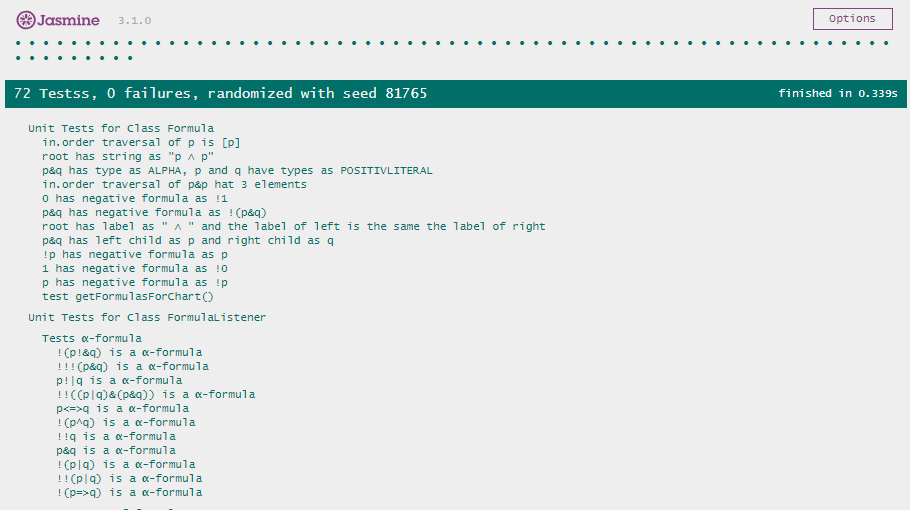
\includegraphics[width=1.0\textwidth]{TestResultModel}
\caption[Testergebnisse des Models]{Ein Teil der Testergebnisse des Models}\label{fig:TestResultModel}
\end{figure}

\begin{figure}[ !h] \centering
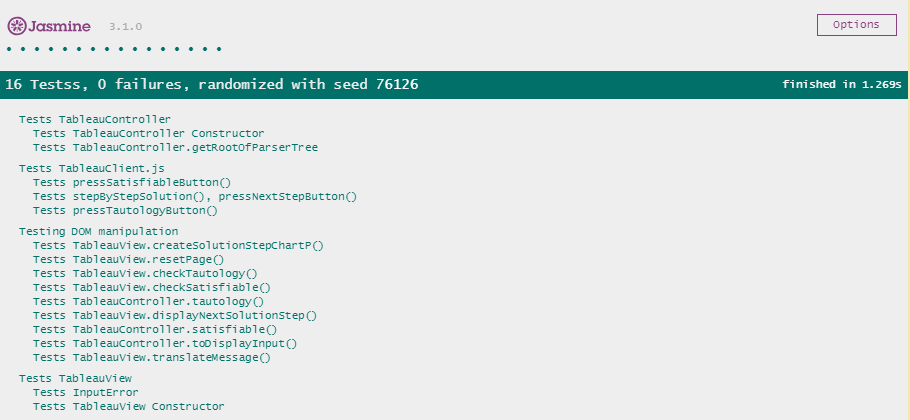
\includegraphics[width=1.0\textwidth]{TestResultControllerView}
\caption[Testergebnisse des Controllers und der View]{Testergebnisse des Controllers und der View}\label{fig:TestResultControllerView}
\end{figure}

Die Tests sind nach der Klasse gruppiert und können dementsprechend zielgerichtet evaluiert werden.
\begin{itemize}

\item \textit{FormulaUnitTest.js}: Enthält 12 Tests für die Klasse \textit{Formula}, wobei alle Methoden der Klasse \textit{Formula} mindestens einmal überprüft werden. Die Methode \textit{getNegativeFormula()} wird mit den Eingabeformeln als Konstante True/False, positive-/negative-Literal, $\alpha $- und  $\beta $-Formel überprüft.

\item \textit{FormulaListenerUnitTest.js}: Enthält 30 Tests. Diese Tests untersuchen die Struktur einer Formel wie linken (\textit{left}) und rechten (\textit{right}) Teilbaum, inhalt (\textit{label}) und Formeltypen (\textit{formulaType}) nachdem sie mithilfe der Klasse \textit{FormulaListener} von Zeichenkette in einen Baum konvertiert wurden. Für jeden Formeltyp (Konstante True/False, positive-/negative-Literal, $ \alpha $- und  $ \beta $-Formel) und für jede Regel der Klassifizierung von $\alpha$- und $\beta$-Formeln wird mindestens eine Formel überprüft.

\item \textit{TableauNodeUnitTest.js}: Enthält 12 Tests für die Klasse \textit{TableauNode}, wobei alle Methoden der Klasse \textit{TableauNode} mindestens einmal überprüft werden. Alle Methoden, die den booleschen Wert zurückgeben, werden mindestens zweimal mit den Rückgabewerten false und true überprüft. Die Methoden \textit{containsOnlyLiterals()}, \textit{containsAComplementaryPairOfLiterals()} und \textit{containsAlphaFormula()} werden mit den Tableau-Knoten, die mit der Menge von Formeln $\{q\}$, $\{p\wedge(q\vee\neg p)\}$, $\{p,q\}$, $\{p,\neg p\}$, $\{\neg p,p\}$, $ \{p,q\vee\neg p\} $, $\{p,\neg p,\neg\neg p\}$, $\{p,1\}$ und $\{q,0\}$ markiert sind, getestet.

\item \textit{TableauForPropositionalLogicUnitTest.js}: Enthält 18 Tests für die Klasse \textit{TableauForPropositionalLogic}, wobei alle Methoden der Klasse \textit{TableauForPropositionalLogic} mindestens einmal überprüft werden. Die Methoden \textit {determineAlphaFormulas()} und \textit{determineBetaFormulas()} werden für jede Regel der Klassifizierung von $\alpha$- und $\beta$-Formeln mindestens einmal überprüft.

\item \textit{TableauControllerandViewUnitTest.js}: Enthält 16 Tests für die Klassen \textit{TableauView}, \textit{TableauController}, \textit{TableauClient.js} und \textit{TableauClient.js} wobei alle Methoden mindestens einmal überprüft werden. Die Methoden \textit { pressSatisfiableButton()} und \textit{pressTautologyButton()} werden für eine syntaktisch korrekte Formel und eine fehlerhafte Formel einmal überprüft.
\end{itemize}


\section{Code Coverage}

\begin{figure}[ !h] \centering
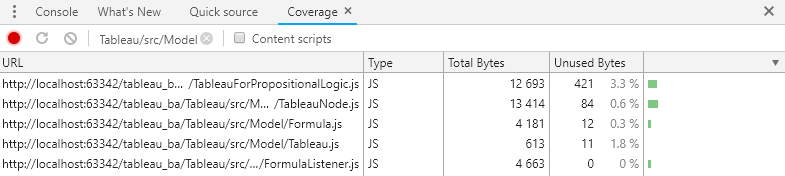
\includegraphics[width=1.0\textwidth]{TestCoverageModel2}
\caption[Code Coverages des Models]{Code Coverages des Models}\label{fig:TestCoverageModel}
\end{figure}

\begin{figure}[ !h] \centering
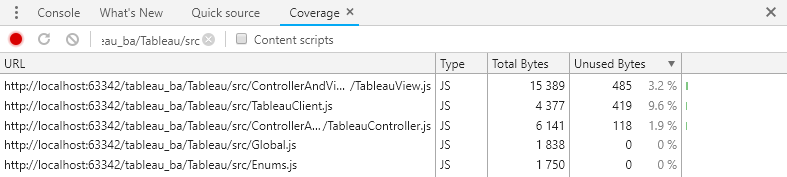
\includegraphics[width=1.0\textwidth]{TestCoverageControllerView5}
\caption[Code Coverages des Controllers und der View]{Code Coverages des Controllers und der View}\label{fig:TestCoverageClientLogik}
\end{figure}

Um eine Code Coverage zu messen, ist ein weiteres Tool notwendig. Es gibt dafür Chrome DevTools, das besteht aus einer Reihe von Webentwicklungs-Tools, die direkt in den Google Chrome-Browser integriert sind. Die neueste DevTools Version (Chrome 59) bietet eine neue Registerkarte ``Coverage'' an. Wenn man eine Seite lädt oder ausführt, erfährt man auf dieser Registerkarte, wie viel Prozent des heruntergeladenen Codes, noch nicht verwendet wurde \cite{Kayce}.
Die Ergebnisse der Codeabdeckung sind unter den Abbildungen \ref{fig:TestCoverageModel} und \ref{fig:TestCoverageClientLogik} zu sehen.

Alle Dateien erfüllen die Mindestgrenze unter Rücksichtnahme, dass das Tool bei \textit{switch-case} und \textit{if-clause}(ohne \textit{else}) nicht richtig ausgewertet werden konnte. Außerdem konnte das Tool auch nicht jedes Event des GUI mit auswerten, deshalb kommt es zu verfälschten Ergebnissen (Abbildung \ref{fig:FehlerCoverage}).

\begin{figure}[ !h] \centering
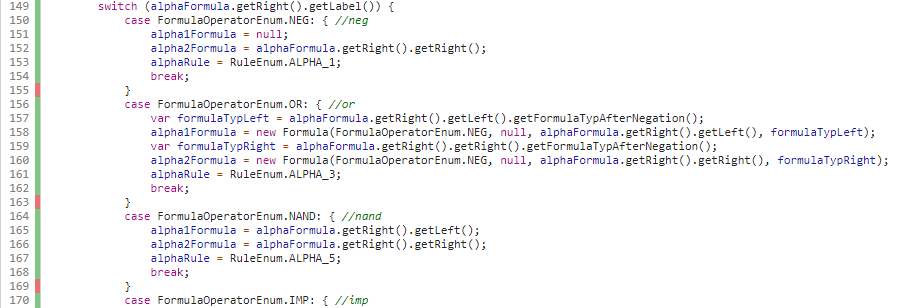
\includegraphics[width=1.0\textwidth]{FehlerCoverage}
\caption[Problem bei CodeCoverages]{Problem bei Code Coverages}
\label{fig:FehlerCoverage}
\end{figure}